%\svnInfo $Id$
%\svnKeyword $HeadURL$

%\documentclass{article}              
%\usepackage{epsfig}
%\begin{document}

\subsubsection{Visualization and Computer Graphics}
\index{Linsen, Lars}

\paragraph{Research Team}
Lars Linsen (Professor),
Sherin Al-Shbat (PhD Student),
Tetyana Ivanovska (PhD Student),
Tran Van Long (PhD Student),
Paul Rosenthal (PhD Student)

\medskip

Lars Linsen is also involved in  ``Smart Systems''
  (Section \ref{???}). % enter

%The Visualization and Computer Graphics Laboratory (VGCL) led by Prof.~Lars
%Linsen is mainly concerned with topics from scientific and information
%visualization  plus some selected topics from computer graphics and geometric
%modeling.
%
%Visualization is an inherently interdisciplinary field with application in many
%different areas. Scientific visualization deals with the visualization of data
%with spatial interpretation such as computer-generated data from numerical
%simulations (physics, chemistry)  or measured data using scanning or sensoring
%techniques (medicine, life sciences, geosciences). The group's efforts are to
%generate visualization methods that can handle large data sets efficiently,
%filter distinct features automatically or interactively, and display the
%relevant information in a comprehensive and intuitive fashion. The research
%focuses on segmentation and isosurface extraction, hierarchical methods,
%multi-variate data visualization, flow and tensor field visualization, and user
%interaction.
%
%Information visualization deals with the visualization of abstract data  with
%no spatial interpretation such as graph- or network-based data (life sciences,
%social sciences) or multi-dimensional data (databases, ecomomics). The group's
%efforts focus on interactive exploration and analysis tools for such abstract
%data.
%
%In the areas of computer graphics and geometric modeling the group's interest
%lies  in point-based methods, multi-resolution surface representation, and
%curves on surfaces.


\paragraph{Highlights} \strut

{\em A Framework for Real-time Volume Visualization of Streaming Scattered
Data.} Scattered data reconstruction algorithms are often computationally
expensive and difficult to implement.  In order to visualize streaming
scattered data, efficient approaches to scattered data reconstruction are
required.  We have developed a general framework for scattered data
interpolation operating on discrete domains.  The key idea for speeding up the
reconstruction over an underlying grid is a re-factorization of the algorithm. 
The re-factorized version is designed such that it easily maps to graphics
hardware architectures  exploiting their performance and parallelism. Moreover,
it naturally extends to applications for streaming data.  As a proof of
concept, we have implemented inverse-distance-weighted interpolation, natural
neighbor interpolation,  and radial Hermite interpolation using our general
framework. In particular, the natural neighbor interpolation  gained a major
speed-up when exploiting geometrical properties of Sibson's interpolant, which
reduces the $d$-dimensional interpolation problem to rendering $d$-dimensional
spheres of known radii and blending them. We have applied the framework to two
kinds of streaming data: progressive scattered data and real-time sensor data
with moving sensors delivering asynchronous measurements.  To account for the
scattered spatial and temporal distribution of streaming sensor data,  we use a
four-dimensional extension of our framework, which elegantly handles
representation of  time-varying data and leads to reconstructions that are
smooth in both space and time.


\begin{figure}[ht]
  \begin{center}
    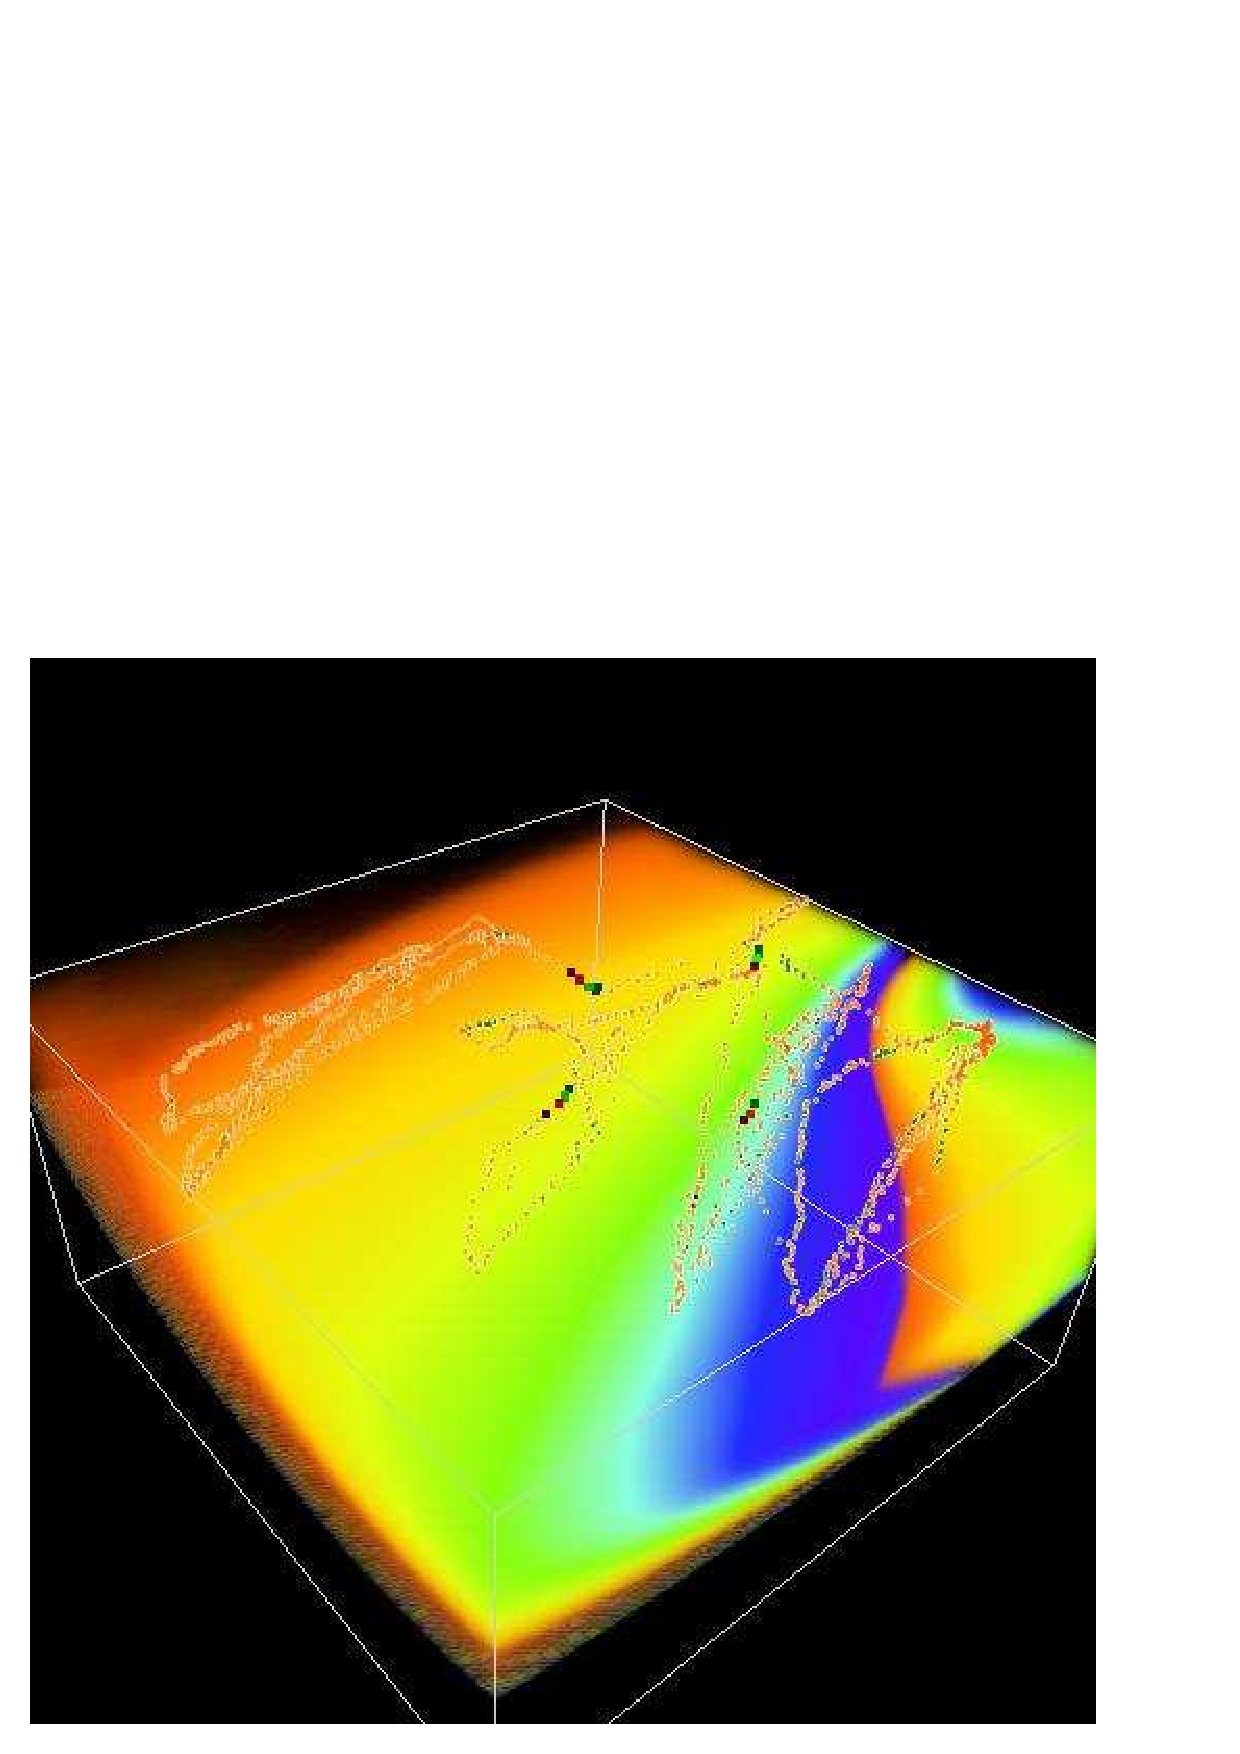
\includegraphics[width=7cm]{MathTheoPhys/Linsen/Linsen_2006_Fig3.pdf}
    \mycaption{Visualization of streaming temperature data in Monterey Bay scattered over time and space. A direct volume rendering of a three-dimensional time-orthogonal hyperplane after reconstruction over a $128 \times 128 \times 64\times 1800$ grid (using natural neighbor interpolation) is shown.}
   \end{center}
\end{figure}

%\end{document}

%%% Local Variables: 
%%% mode: latex
%%% TeX-master: report
%%% End: 
